% ===============================================================================
% = LaTeX Beamer Template des Arbeitsbereichs Sicherheit in verteilten Systemem
% = (c) 2016 Prof. Dr. Hannes Federrath, Uni Hamburg, Fachbereich Informatik
% = https://svs.informatik.uni-hamburg.de
% =
% = Weitgehend in Übereinstimmung mit dem Corporate Design 2016 der UHH:
% = https://www.uni-hamburg.de/beschaeftigtenportal/services/oeffentlichkeitsarbeit/corporate-design.html
% =
% ===============================================================================
%
\documentclass[t]{beamer}
% Option t              Place text of slides at the (vertical) top of the slides.
% Option handout        Ein PDF ohne Pausen und Overlayeffekte erzeugen.
% Option aspectratio=43 169 => 16:9, 1610 => 16:10, 43 => 4:3
\usepackage[utf8]{inputenc}
\usepackage[english]{babel}
\usepackage{graphicx,xcolor}
\usepackage{minted}
\usepackage[T1]{fontenc} % 8-Bit-Zeichen; ermöglicht korrektes Kopieren von Umlauten aus dem pdf
\usepackage[absolute,overlay]{textpos}
  \setlength{\TPHorizModule}{1mm}
  \setlength{\TPVertModule}{1mm}
\graphicspath{{graphs/}}

\setcounter{tocdepth}{1}

% SVS-Theme benutzen
\usetheme{svs2016}


% =============================
% = Ab hier Inhalte ändern...
% =============================

\title[Privacy Implications of Exposing Git Metadata]
{Privacy Implications of Exposing Git Metadata}
\author[Beer]{Arne Beer \\ \footnotesize Matriculation number: 6489196}
\subject{Computer Science}

\begin{document}

\begin{frame}[plain]
    \maketitle
\end{frame}

\begin{frame}
    \frametitle{Table of Contents}
	% Die Gliederung erscheit nach erneutem Übersetzen korrekt.
	\tableofcontents
\end{frame}

\section{Introduction}
\begin{frame}
    \frametitle{Topic}
    \begin{center}
        \vspace{1cm}
        \begin{block}{Main topic of the thesis}
            Is it possible to extract personal information?
        \end{block}
    \end{center}
\end{frame}

\begin{frame}
    \frametitle{Motivation}
    \vspace{5mm}
    \begin{center}
        
\includegraphics[scale=0.15]{./pic/git-logo.png}
    \end{center}
    \begin{itemize}
        \item Used in most projects for version control
        \pause{}
        \item No obvious leak of personal information
        \pause{}
        \item Leaked information could be used maliciously
    \end{itemize}
\end{frame}

\begin{frame}
    \frametitle{Leading Question and Goals}
    \vspace{1cm}
    \begin{itemize}
        \item Feasibility of scanning repositories
        \item Possible extraction of interesting information
        \item Analyse possible attack goals
    \end{itemize}
\end{frame}

\section{Data}

\begin{frame}[fragile]
    \frametitle{Git Metadata}
    \begin{minted}{text}
tree      cd7d001b696db430b898b75c633686067e6f0b76
parent    c19b969705e5eae0ccca2cde1d8a98be1a1eab4d
author    Arne Beer <contact@arne.beer> 1513434723 +0100
committer Arne Beer <contact@arne.beer> 1513434723 +0100

Chapter 2, acronyms
    \end{minted}

    \begin{itemize}
        \item Parent commit file reference
        \item Tree file reference
        \item Name and email
        \item Commit timestamp with UTC offset
    \end{itemize}
\end{frame}

\begin{frame}
    \frametitle{Why Github?}
    \begin{center}
        
\includegraphics[scale=0.12]{./pic/github-logo.png}
    \end{center}

    \begin{itemize}
        \item Largest accumulation of open-source Git repositories
        \pause{}
        \item Great API
        \pause{}
        \item Organizations
        \pause{}
        \item Allows exploration for collecting user repositories.
        \begin{itemize}
            \item Stars
            \item Following
        \end{itemize}
    \end{itemize}
\end{frame}

\begin{frame}
    \frametitle{Gitalizer}
    \begin{center}
        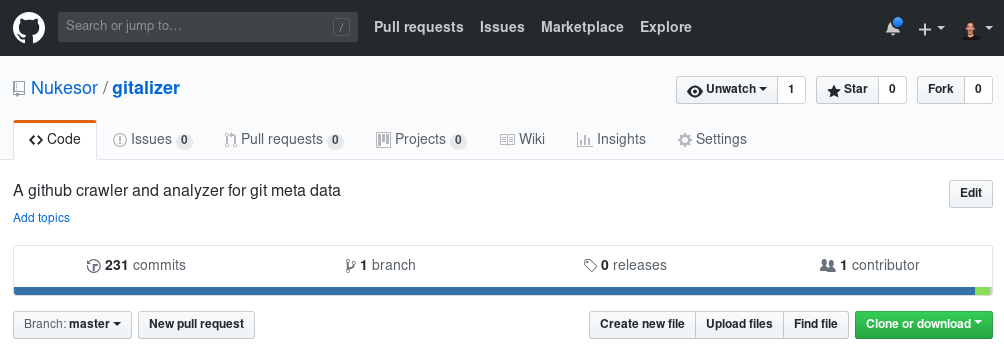
\includegraphics[scale=0.30]{./pic/gitalizer-github.png}
    \end{center}

    \begin{itemize}
        \item Gathers data from Github
        \item Uses user or organization as entry point
        \item Highly optimized
    \end{itemize}
\end{frame}

\section{Research}
\begin{frame}
    \frametitle{Three Chosen Attacks}
    \vspace{1cm}
    \begin{itemize}
        \item Holiday and sick leave detection
        \pause{}
        \item Sleep rhythm and working hours
        \pause{}
        \item Geographic location
    \end{itemize}
\end{frame}

\begin{frame}
    \frametitle{Holiday and Sick Leave: Goals}
    \vspace{1cm}
    \begin{itemize}
        \item Detect holiday or sick leave
        \pause{}
        \item Detect other anomalies
        \pause{}
        \item Good visualization
    \end{itemize}
\end{frame}

\begin{frame}
    \frametitle{Methodology}
    \vspace{1cm}
    \begin{itemize}
        \item All commits of one contributor
        \item Find regular work pattern
        \item Detect unregular work pattern
        \item Detect anomalies
    \end{itemize}
\end{frame}

\begin{frame}
    \frametitle{Example}
    \begin{figure}[H]
        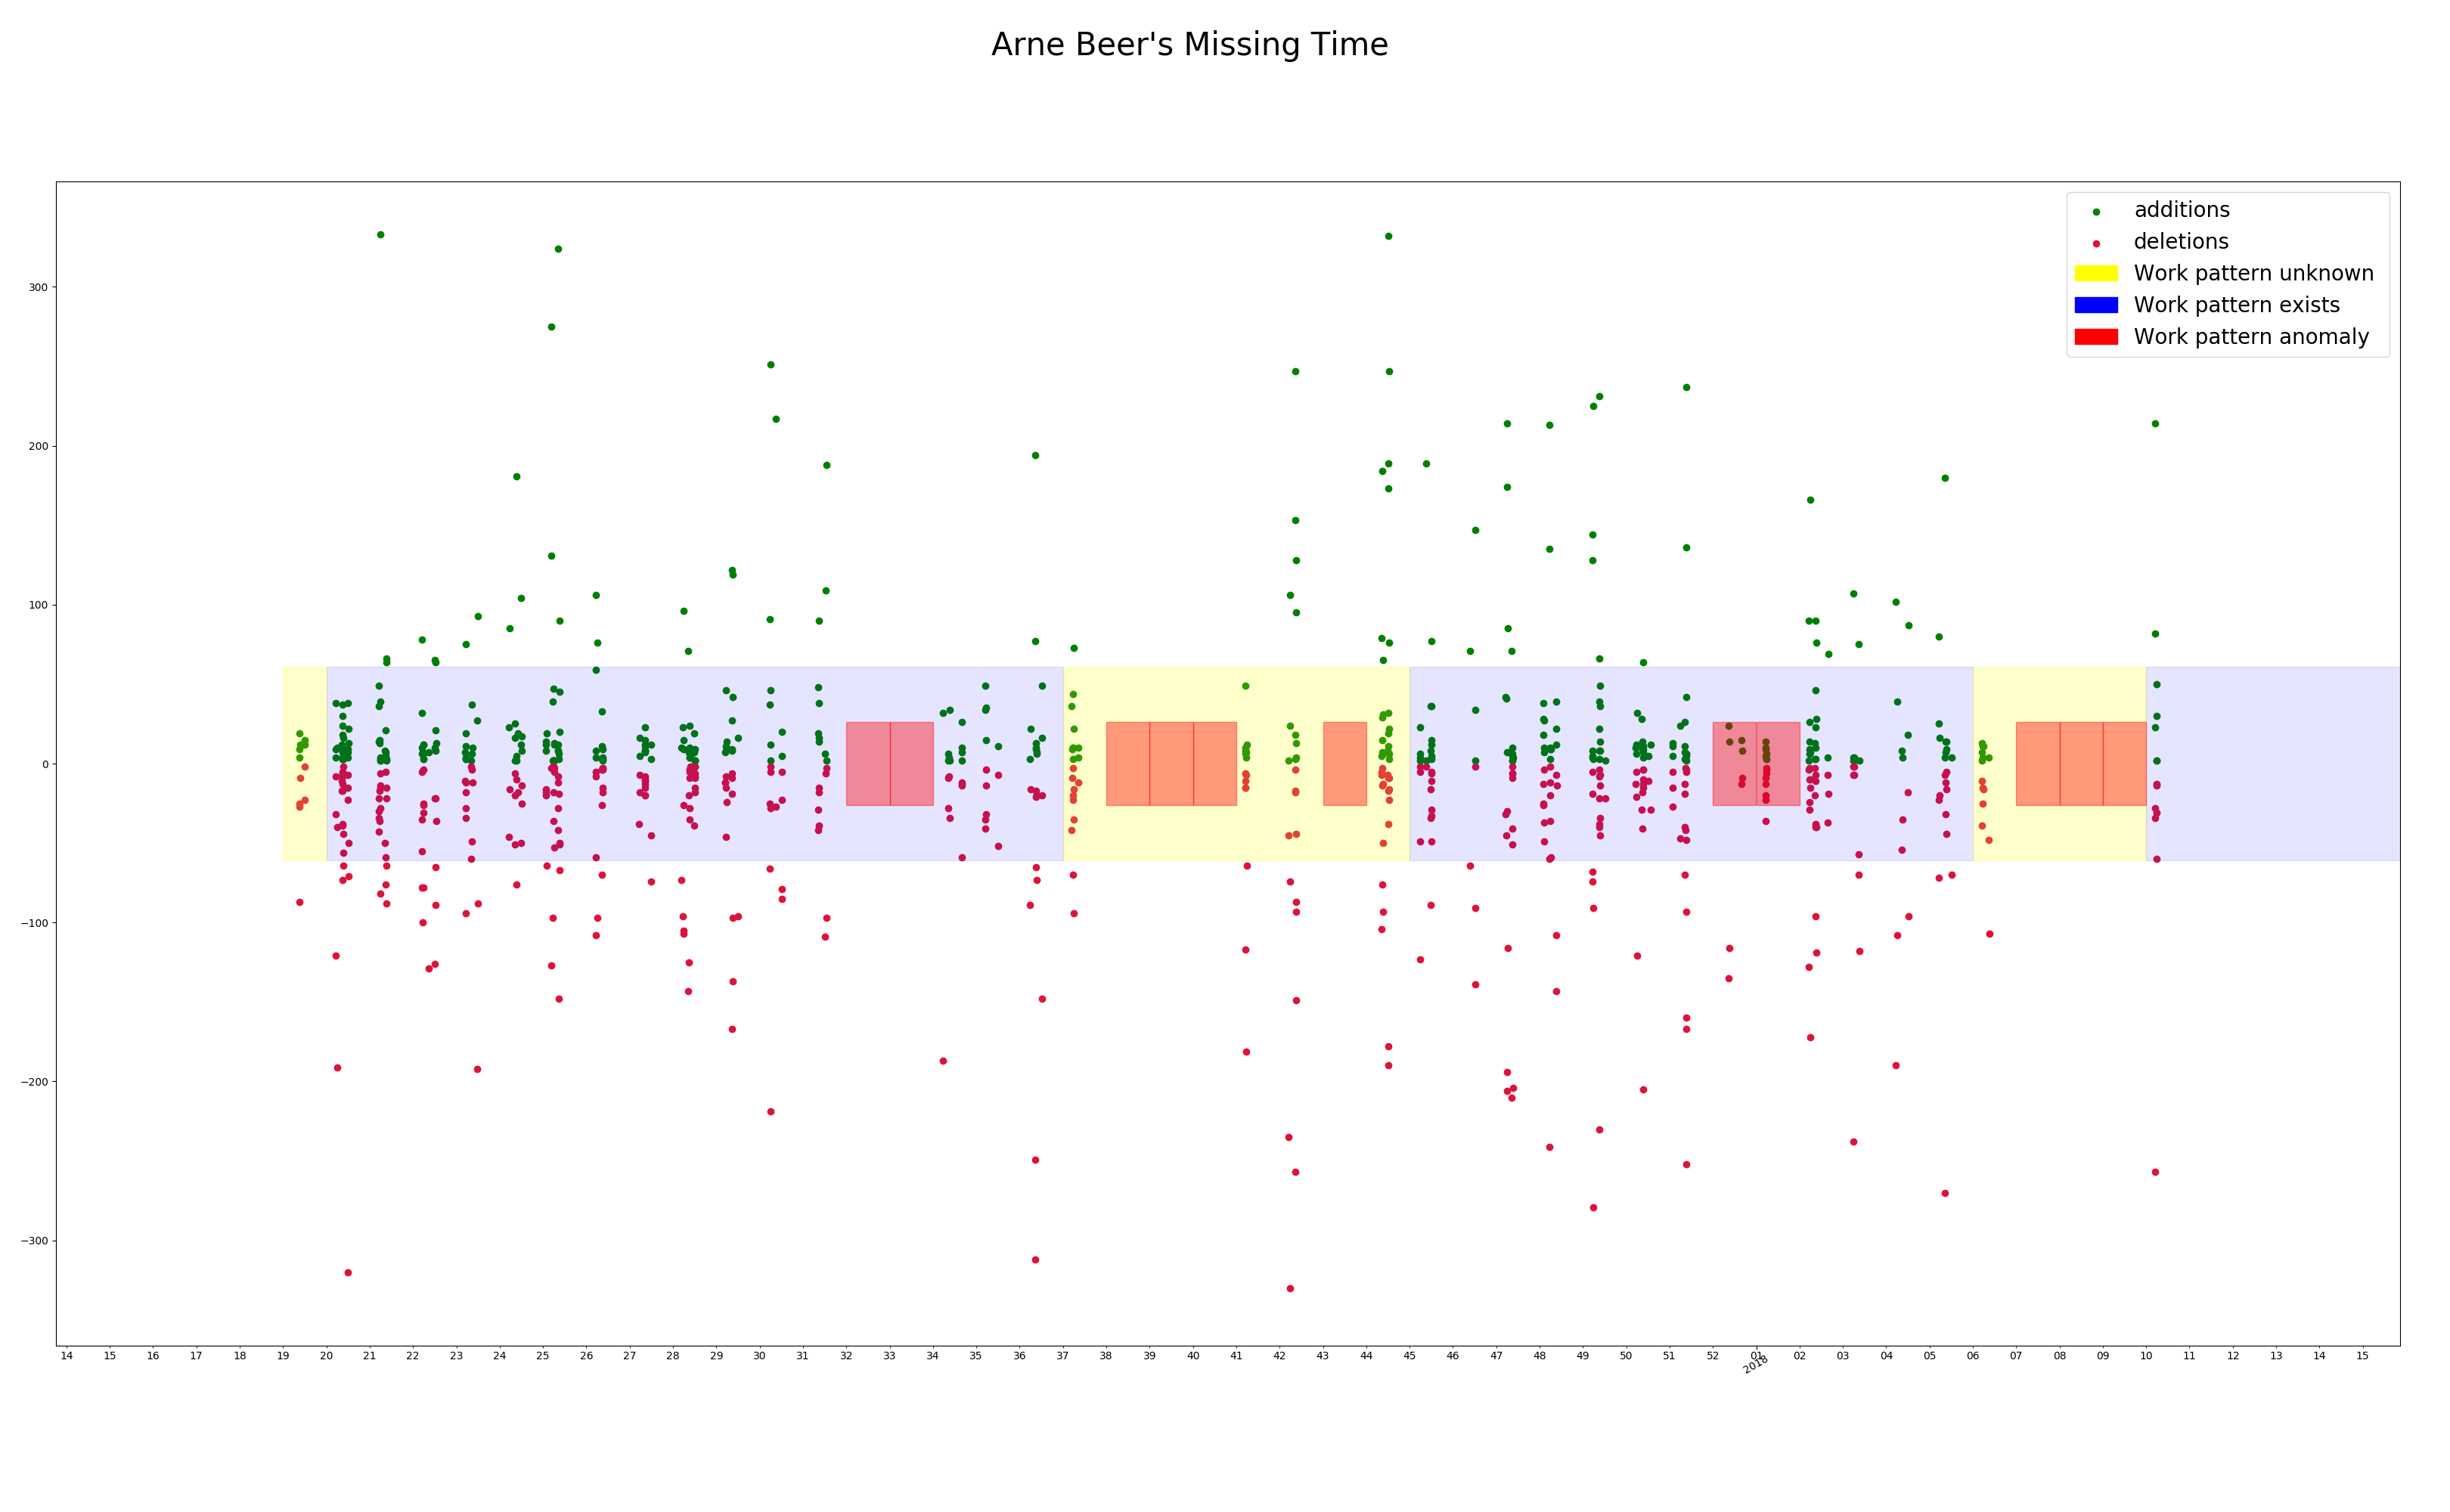
\includegraphics[scale=0.115]{analysis/work-time-analysis}
        \centering
        \caption{Holiday and Sick leave visualization}
    \end{figure}
\end{frame}

\begin{frame}
    \frametitle{Results}
    \vspace{1cm}
    \begin{itemize}
        \item Tested in a small company
        \pause{}
        \item Accurate holiday detection
        \pause{}
        \item Some false positives
        \pause{}
        \item Other anomaly detection needs interpretation
    \end{itemize}
\end{frame}

\begin{frame}
    \frametitle{Sleep Rhythm and Working Hours: Goals}
    \vspace{1cm}
    \begin{itemize}
        \item Good visualization
        \pause{}
        \item Check visibility of sleep rhythm
        \pause{}
        \item Check link to working behavior
    \end{itemize}
\end{frame}

\begin{frame}
    \frametitle{Example}
    \vspace{1cm}
    \begin{figure}[H]
        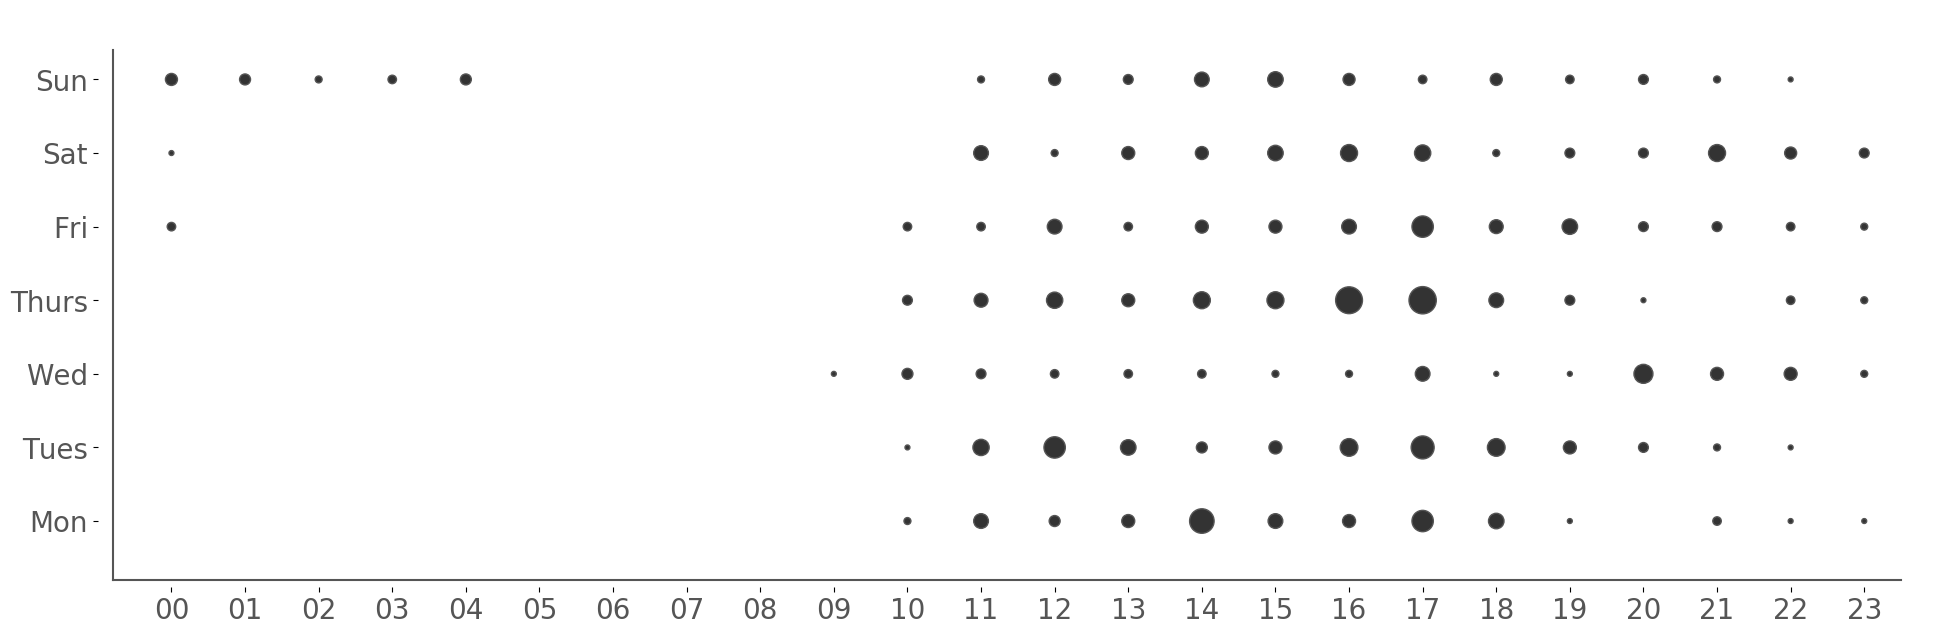
\includegraphics[scale=0.22]{analysis/ordered-punchcard}
        \centering
        \caption{Regular sleep rhythm}
    \end{figure}
\end{frame}

\begin{frame}
    \frametitle{Example}
    \vspace{1cm}
    \begin{figure}[H]
        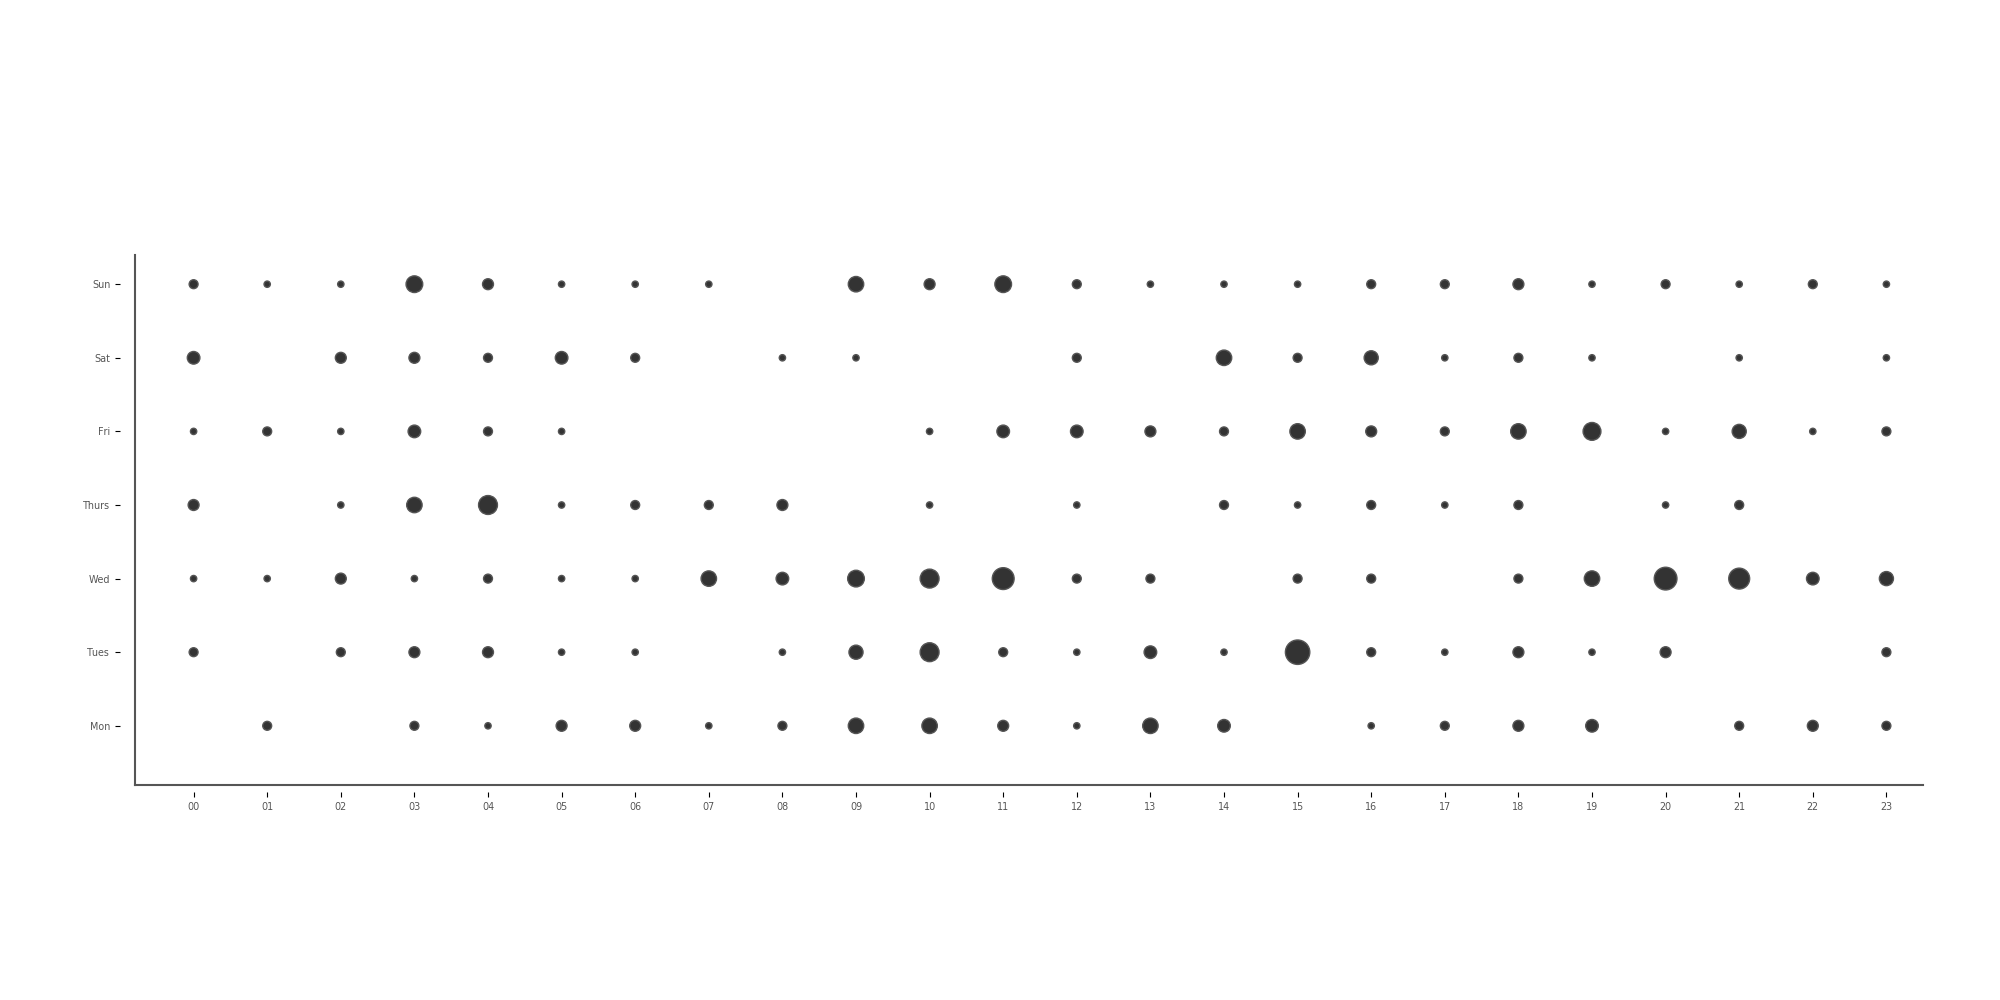
\includegraphics[scale=0.22]{analysis/random-punchcard}
        \centering
        \caption{Person without a sleep rhythm}
    \end{figure}
\end{frame}

\begin{frame}
    \frametitle{Example}
    \vspace{1cm}
    \begin{figure}[H]
        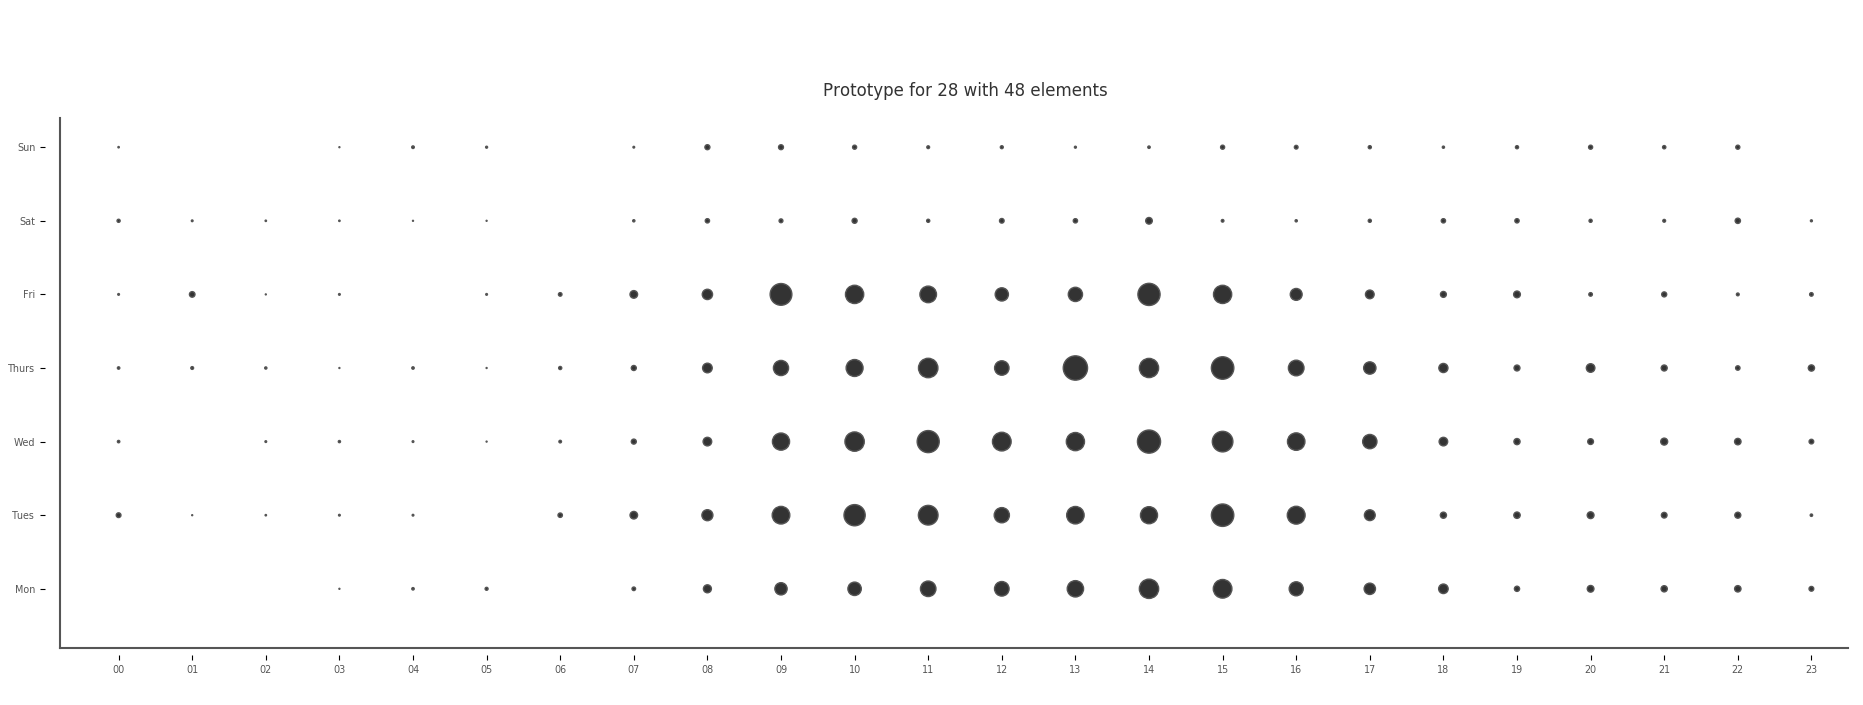
\includegraphics[scale=0.22]{analysis-affinity/28}
        \centering
        \caption{Normal working hour punchcard}
    \end{figure}
\end{frame}

\begin{frame}
    \frametitle{Results}
    \vspace{1cm}
    \begin{itemize}
        \item Tested for correctness in small test group
        \pause{}
        \item Sleep rhythm rather accurate
        \pause{}
        \item Allows to guess working behaviour
    \end{itemize}
\end{frame}

\begin{frame}
    \frametitle{Geographic Location: Goals}
    \vspace{1cm}
    \begin{itemize}
        \item Detect home country
        \pause{}
        \item Detect holiday destinations
    \end{itemize}
\end{frame}

\begin{frame}
    \frametitle{Example}
    \begin{figure}[H]
        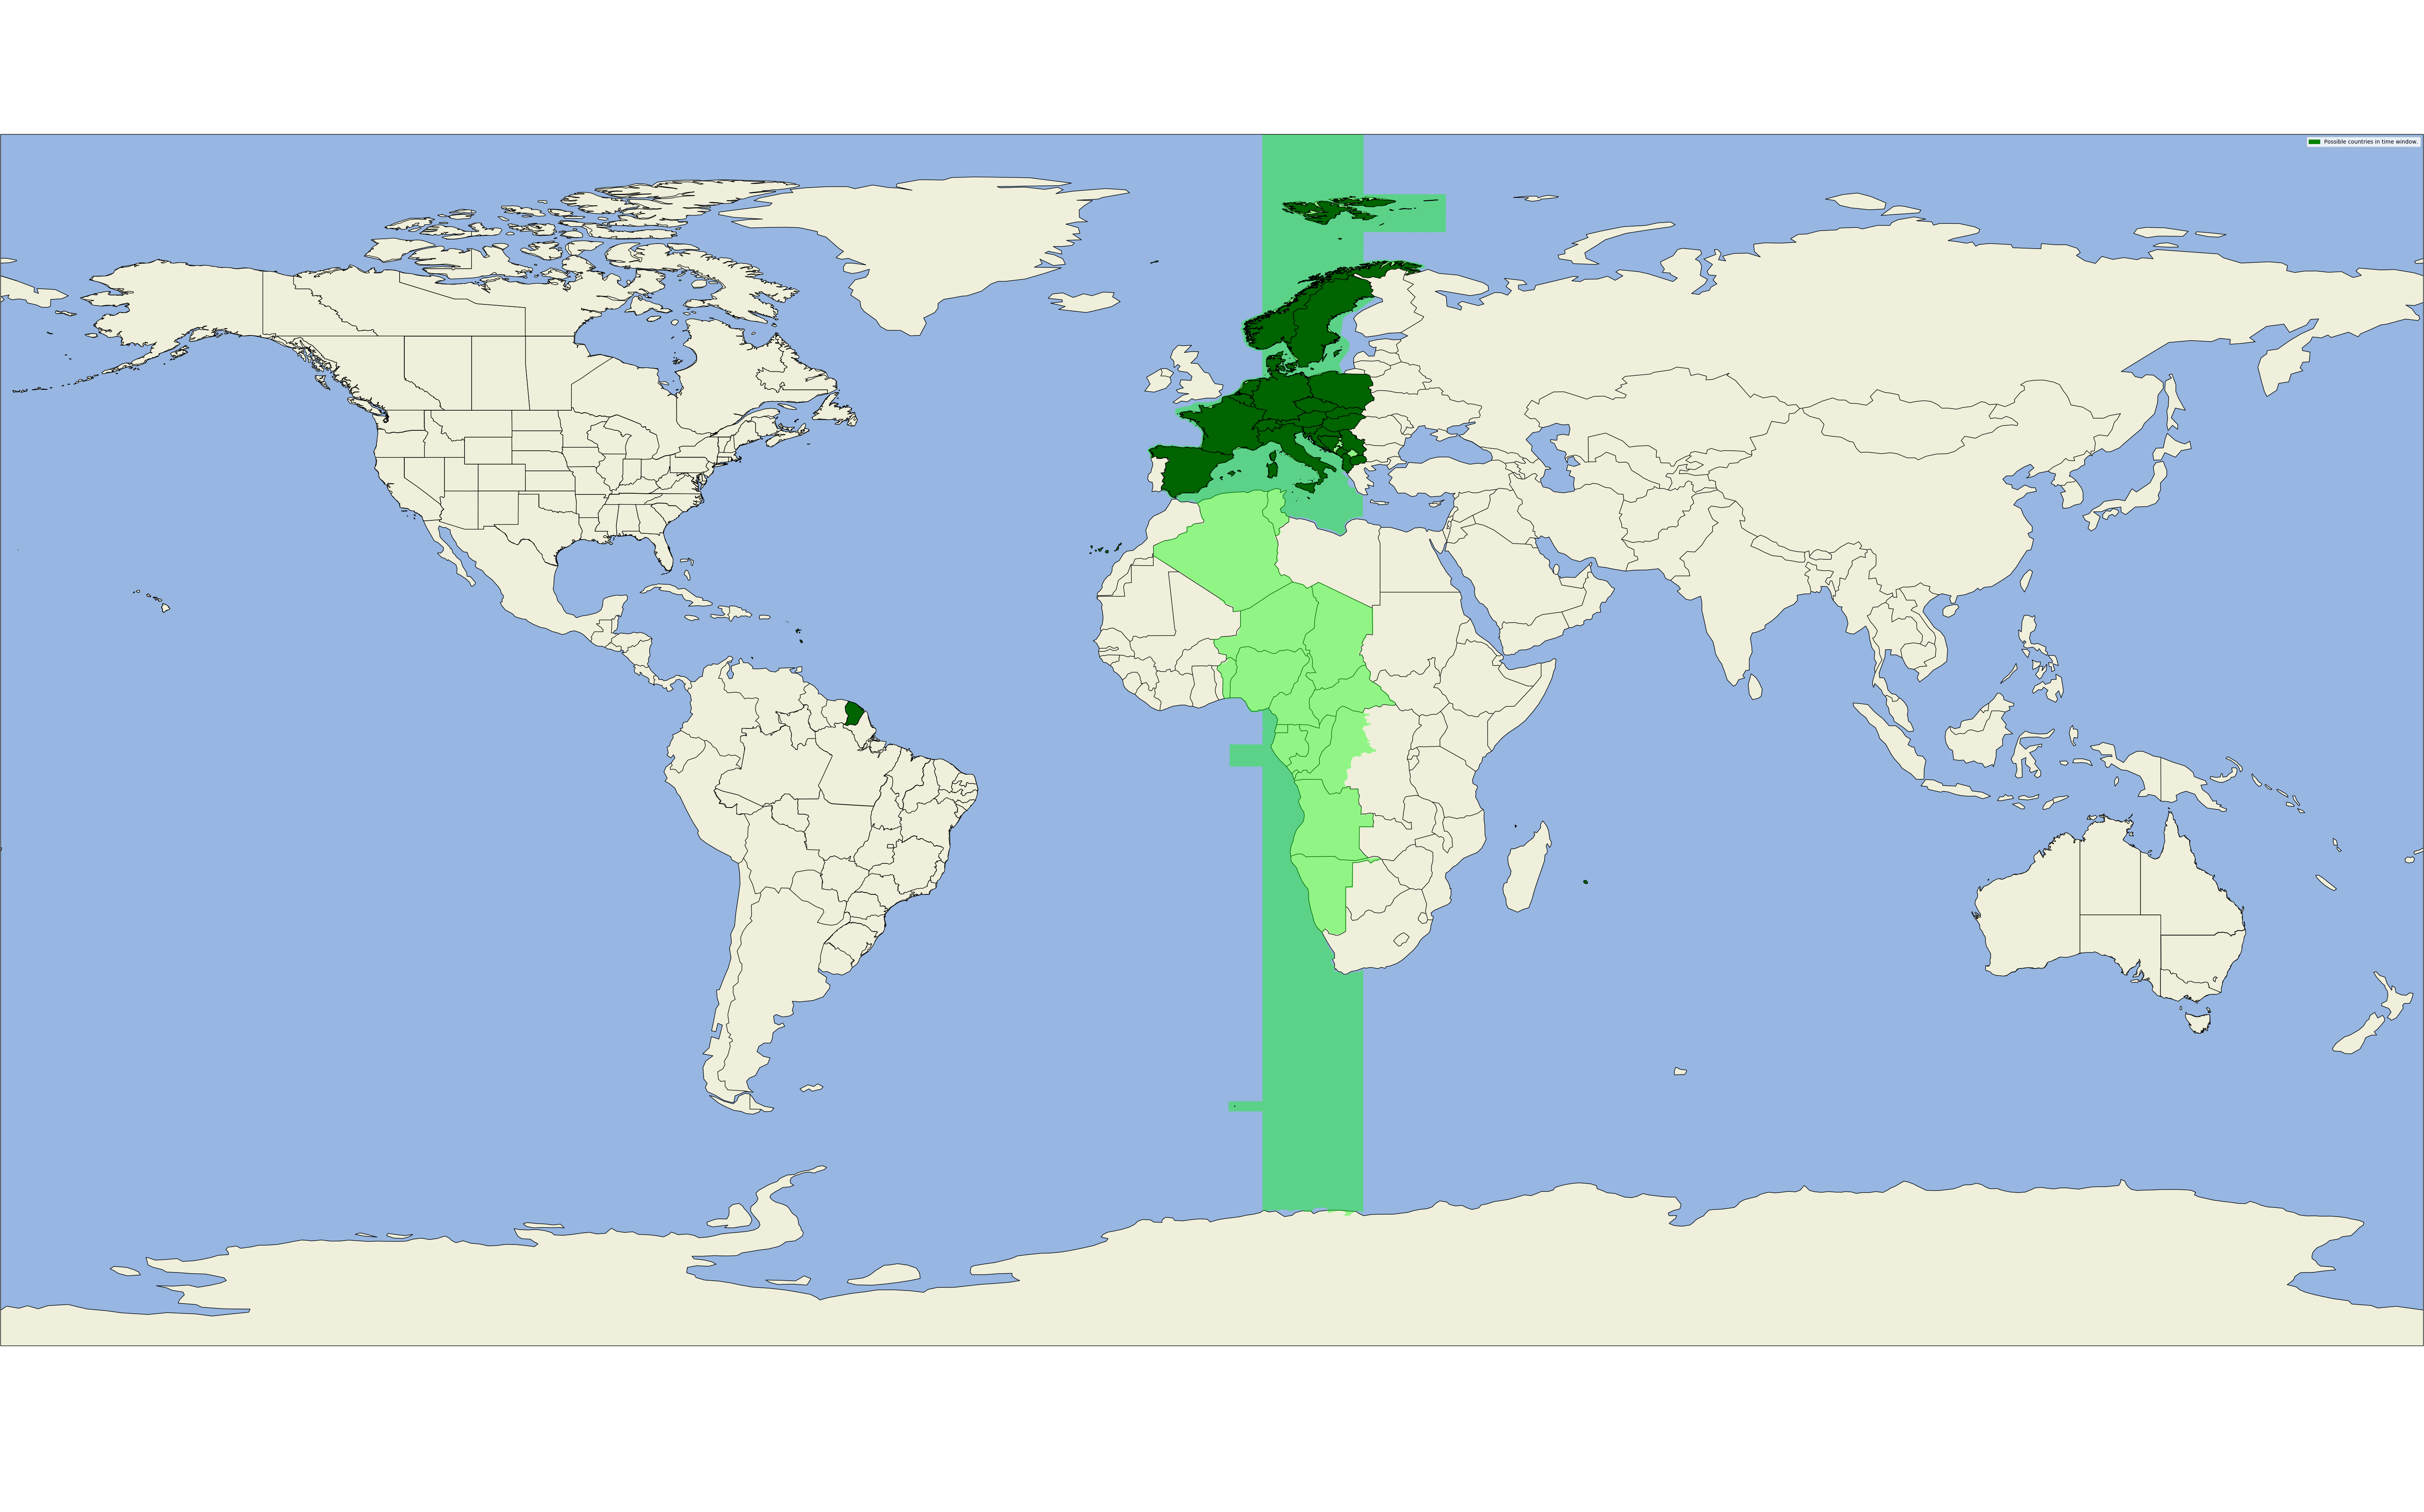
\includegraphics[scale=0.06]{analysis/author-home-location}
        \centering
        \caption{Home location analysis}
    \end{figure}
\end{frame}

\begin{frame}
    \frametitle{Methodology}
    \vspace{1cm}
    \begin{itemize}
        \item All commits of one contributor
        \item Possible timezones/countries for offset
        \item Daylight Savings Time
        \item Detect timezone switches
    \end{itemize}
\end{frame}

\begin{frame}
    \frametitle{Results}
    \vspace{1cm}
    \begin{itemize}
        \item Good detection of home country (82\%)
        \pause{}
        \item Holiday not checked
        \pause{}
        \item Needs better libraries
    \end{itemize}
\end{frame}

\section{Conclusion and Outlook}
\begin{frame}
    \frametitle{Conclusion}
    \vspace{1cm}
    \begin{itemize}
        \item Recall the goal: Is it possible to extract personal information
        \pause{}
        \item It is possible to extract further personal information
        \pause{}
        \item Simple goals, but already offers possibly sensitive information
    \end{itemize}
\end{frame}

\begin{frame}
    \frametitle{Outlook}
    \vspace{1cm}
    \begin{itemize}
        \item Many more complex and promising attacks
        \pause{}
        \item It could become a problem
        \pause{}
        \item Methodologies to obfuscate data
    \end{itemize}
\end{frame}


\begin{frame}
    \frametitle{Fin}
    Thank you for your attention.
\end{frame}

\end{document}
